\chapter{\noun{Data Flows}   }
\section{\noun{Use Cases} }

%\begin{figure}
    %\centering
    %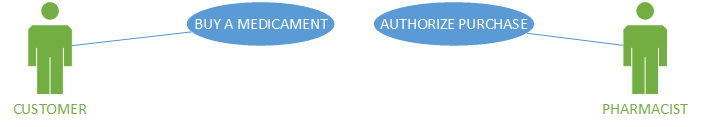
\includegraphics[width=1\textwidth]{use-case.png}
    %\caption{General use case}
    %\label{fig:usecase}
%\end{figure} 

The way prescriptions are currently processed is vulnerable to many threats, and brings many inconveniences. The most important ones are listed below.


\begin{enumerate}
\item{\textbf{System:}}
\begin{itemize}
\item{\textbf{pharmacist's verification} - system is ableto check that pharmacist has permissions to sell the drugs;}
\item{\textbf{buyer's verification} - system is able to check that the buye's card is valid and entered PIN number was correct;}
\item{\textbf{prescriptions update} - system can change the state of prescriptions(to either \textquoteleft{}bought\textquoteright{} or \textquoteleft{}invalid\textquoteright{}) or attach additional info to them, like the fact that drug\textquoteright{}s substitute was sold instead of prescribed one;}
\end{itemize}


\item{\textbf{Pharmacist:}}
\begin{itemize}
\item {\textbf{reading available prescriptions} - a pharmacist is able to seebuyer\textquoteright{}s prescriptions}
\item{\textbf{modifying the prescriptions} - a pharmacist is able to update the prescriptions (changing their state/attaching info that substitute was sold instead)}
\item{\textbf{signing the prescriptions} - a pharmacist is able to sign prescription to confirm that he\textquoteright{}s the one who sold them}
\end{itemize}
\item{\textbf{Customer:}}
\begin{itemize}
\item {\textbf{reading available prescriptions} - a customer is able to see/select prescriptions that haven\textquoteright{}t yet been bought}
\item{\textbf{confirming pharmacist\textquoteright{}s changes} - a customer is obliged to confirm possible changes made to the prescriptions by the pharmacist}
\item{\textbf{signing the prescriptions} - a customer is able to sign prescription
to confirm that he got the certain medicines}
\end{itemize}
\end{enumerate}


\begin{figure}[h]
    \centering
    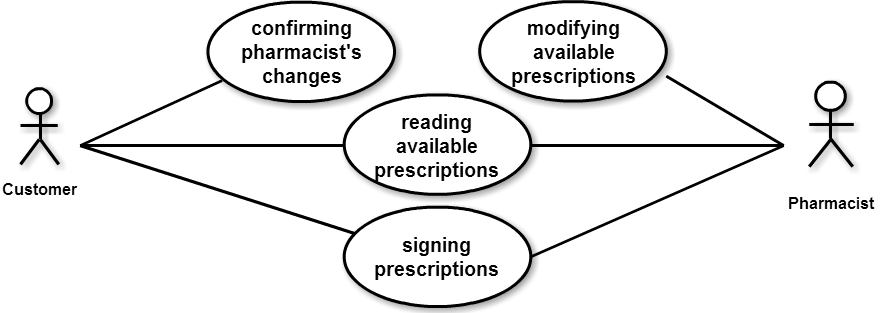
\includegraphics[width=0.75\textheight]{use-case-2.png}
    \caption{Patient's and pharmacist's use cases}
    \label{fig:usecase}
\end{figure} 

\begin{figure}[h]
    \centering
    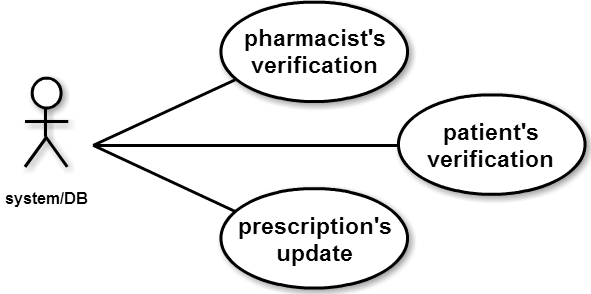
\includegraphics[width=0.45\textheight]{use-case-1.png}
    \caption{System's use cases}
    \label{fig:usecase}
\end{figure} 


\newpage
\section{\noun{Scenario}}

\begin{enumerate}
  \item Customer inserts his card into the reader and enters PIN number.
  \begin{enumerate}
	\item System checks whether PIN is correct (if it is not, an appropriate message is displayed and the process cannot be continued).
  \end{enumerate}
  \item Terminal displays list of active prescriptions to both buyer and pharmacist.
  \item Buyer selects prescriptions to buy.
  \item Pharmacist inserts his card into his reader and authenticates himself to the system (assuming that the card is not already inserted).
  \begin{enumerate}
	\item  If authentication is not possible (eg. card of the pharmacist is invalid), an appropriate error message appears on the screen and the process can't be continued.
  \end{enumerate}
  \item The pharmacist marks prescriptions selected by the customers as 'to be bought'.
  \item System checks whether prescriptions have already been bought.
  \item System verifies validity of prescriptions (expiration date, credentials of the doctor etc.)
 \begin{enumerate}
	\item If some prescriptions are invalid, an appropriate message appears on the screen and system marks the prescriptions as 'invalid'.
  \end{enumerate}
  \item  If the drug from the prescription is not available (or the buyer does not want it for some reason), pharmacist can instead sell a substitute. For that, he is able to write information about selling a substitute to the system.
  \item Buyer confirms the prescriptions to be bought (including possible substitute replacements).
  \item Pharmacist gives the drugs to the buyer, confirms the selling and the system marks the prescriptions as 'bought'.
  \item  Buyer takes the drugs and removes his card from the reader.
\end{enumerate}

 If the customer's or pharmacist's card is removed from the reader before the step 10, the process is aborted and the initial state of the prescriptions is not changed.
\newpage
\pagenumbering{gobble}
\fboxsep=5mm%padding thickness

\begin{figure}
    \centering
    \hspace*{-0.4in}
    \fbox{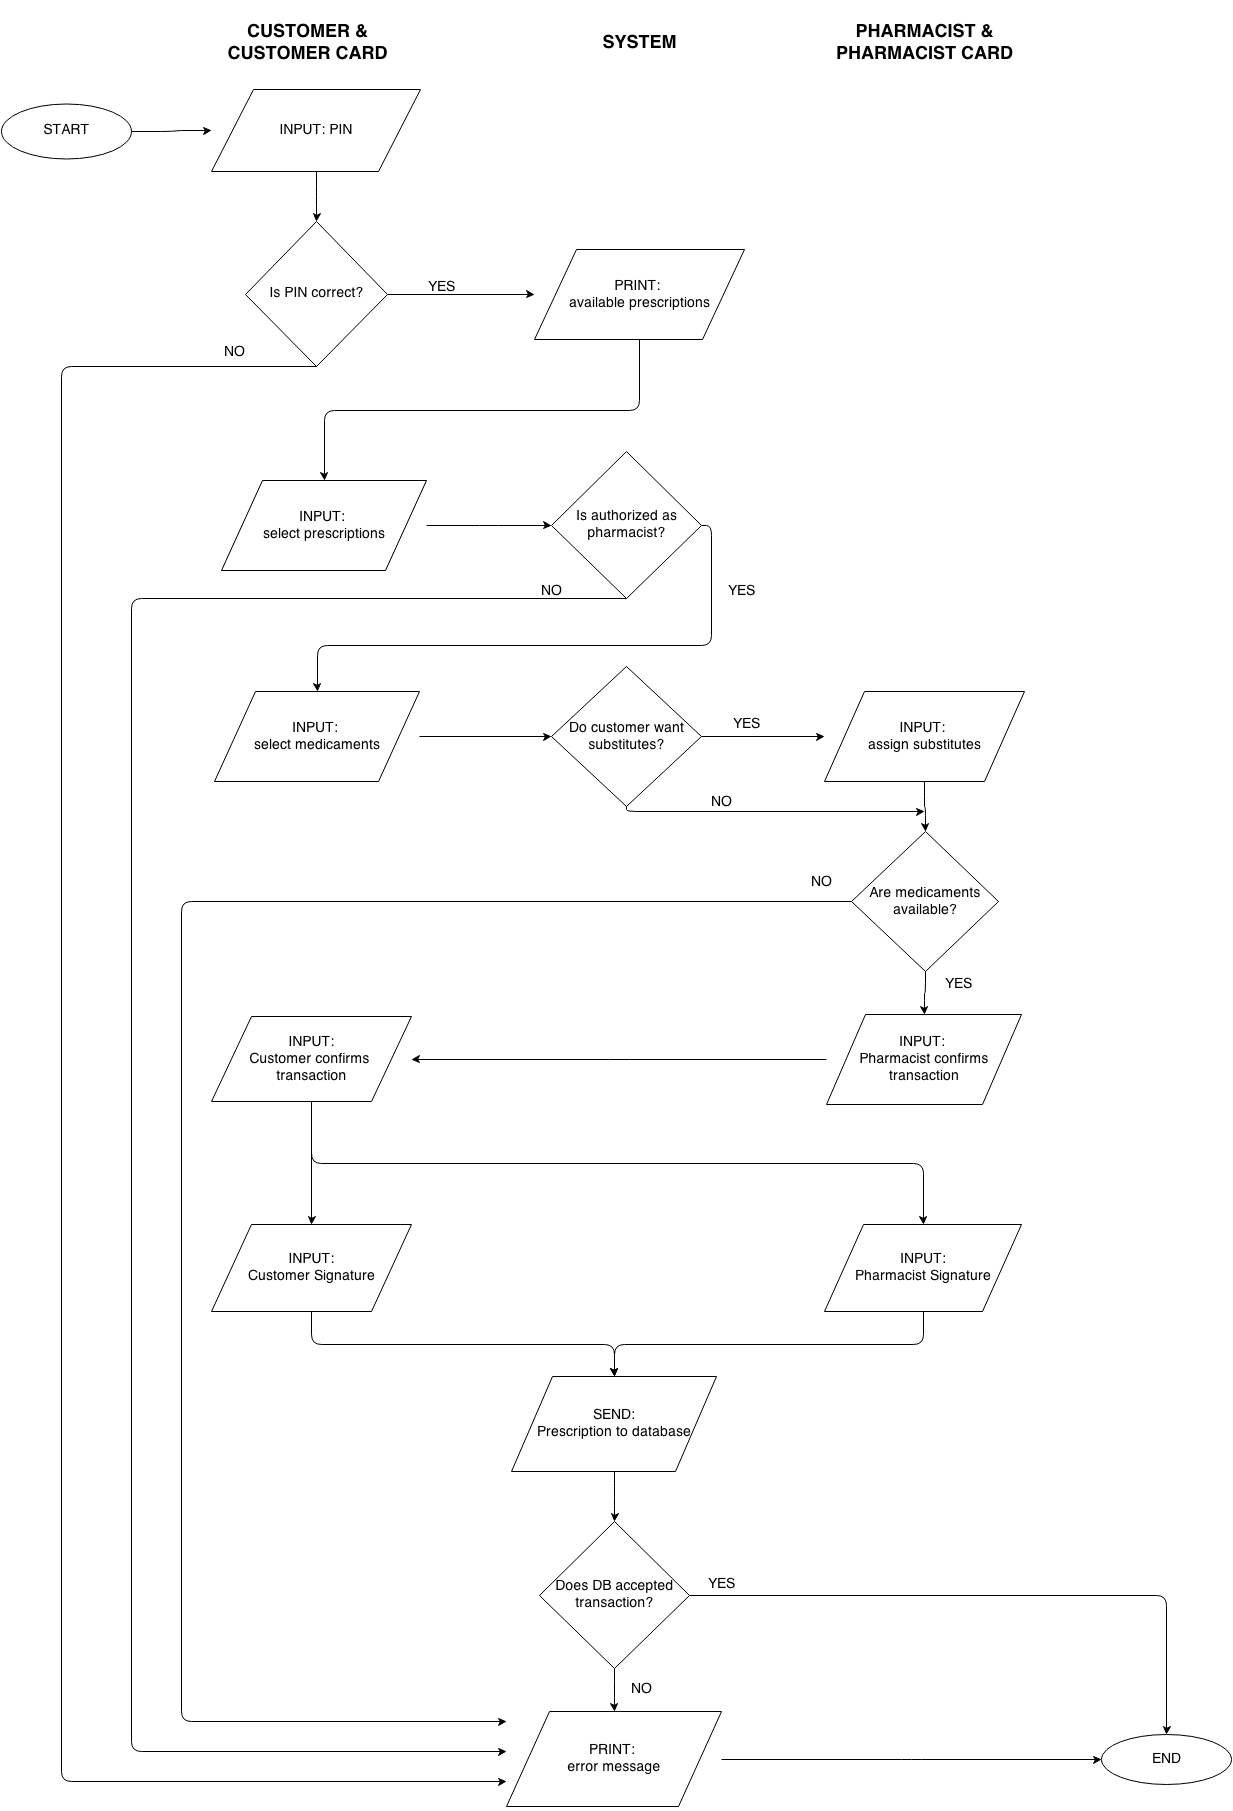
\includegraphics[width=0.78\textheight]{flow-chart.png}}
    \caption{Flow chart}
    \label{fig:flowchart}
\end{figure} 

\pagenumbering{arabic}
\setcounter{page}{100}

